\chapter{Modelación para la simulación de enfermedades transmitidas por vectores}\label{chapter:proposal}
\section{Vectores}
Un vector es un organismo vivo, como un insecto o artrópodo, que puede transmitir un agente 
infeccioso, como un virus, una bacteria o un parásito, de un huésped infectado a un huésped 
susceptible. Los vectores pueden actuar como intermediarios en la transmisión de enfermedades, 
ya sea mecánicamente, a través de la contaminación de alimentos o superficies con el agente 
infeccioso, o biológicamente, cuando el agente infeccioso se replica y multiplica dentro del 
vector antes de ser transmitido a un nuevo huésped. Los vectores son una parte integral de la 
epidemiología de muchas enfermedades infecciosas y desempeñan un papel crucial en su mantenimiento 
y propagación.\autocite{Reisen2010}\\

Según la OMS, las enfermedades airborne (arthropod-borne) representan 17 por ciento del total de 
las enfermedades infecciosas en el mundo, con 1,000 millones de casos y un millón de defunciones 
anuales \autocite{OMS2020}. Los vectores biológicos más comunes son los insectos hematófagos que 
al alimentarse de la sangre de un portador infectado, ingieren microorganismos patógenos que 
posteriormente inoculan a otro individuo.\\

\textbf{Características generales de los vectores:}\autocite{OMS2020}
\begin{enumerate}
    \item Especies específicas: Los vectores suelen ser especies específicas de insectos, 
    artrópodos u otros organismos. Por ejemplo, los mosquitos, las garrapatas, las pulgas y los 
    flebótomos son ejemplos comunes de vectores. 
    \item Capacidad de transmitir enfermedades: Los vectores tienen la capacidad de transmitir 
    agentes patógenos, como virus, bacterias o parásitos, de un huésped infectado a un huésped 
    susceptible. Esto puede ocurrir a través de la picadura o el contacto con el vector.
    \item Dependencia de los huéspedes: Los vectores dependen de la sangre u otros recursos de 
    sus huéspedes para alimentarse y reproducirse. Por lo tanto, su presencia y actividad están 
    estrechamente relacionadas con la disponibilidad de los huéspedes adecuados.
\end{enumerate}
\subsection{Enfermedades Transmitidas por Vectores (ETV)}
Entre las ETV que han aumentado en las últimas décadas están el 
paludismo o malaria, la fiebre hemorrágica por dengue, la esquistosomiasis, la tripanosomiasis americana 
o enfermedad de Chagas, la tripanosomiasis africana o enfermedad del sueño, la leishmaniasis, la fiebre 
amarilla, la encefalitis japonesa, la fiebre por zika  y la fiebre por chikungunya. Otras ETV menos frecuentes 
son la borreliosis o enfermedad de  Lyme y la enfermedad por el  virus del oeste del Nilo.\autocite{Torres2020}\\

\begin{figure}[htb]
    \centering
    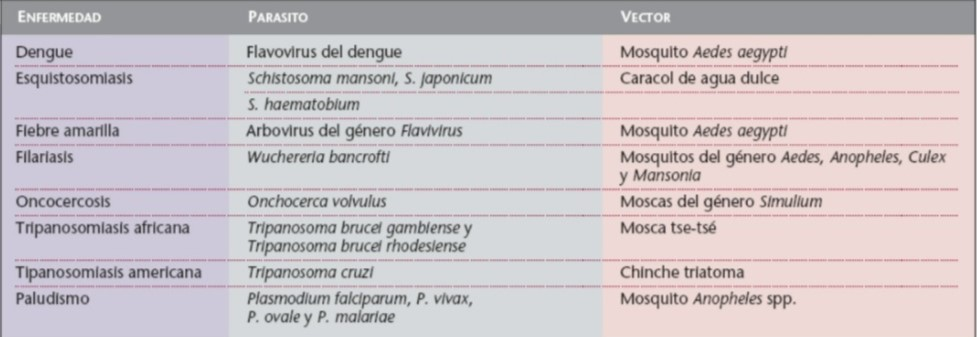
\includegraphics[width=1\textwidth]{Graphics/EnfVec.jpeg}
    \caption{Algunas enfermedades transmitidas por vectores.\autocite{Tercero2008}}
\end{figure}

La distribución de las ETV está vinculada a una serie de factores complejos 
de naturaleza demográfica, ecológica, medioambiental y social. Estos factores incluyen:
\begin{enumerate}
    \item El fenómeno del calentamiento global y el consiguiente cambio climático, que permite la adaptación de los vectores a nuevas altitudes y la propagación de patógenos en regiones previamente no afectadas.
    \item La sobrepoblación y el hacinamiento en áreas específicas, lo cual propicia un aumento en la presencia de vectores y hospederos susceptibles, como perros y gatos.
    \item La densidad de población de los artrópodos vectores y la diversidad de especies presentes en un área determinada.
    \item La falta de medidas adecuadas de higiene a nivel personal, en viviendas y en comunidades.
    \item El incremento en la frecuencia y distancia de los viajes internacionales.
    \item La existencia de marginación, pobreza y urbanización descontrolada.
\end{enumerate}

Actualmente, la enfermedad transmitida por vector con mayor crecimiento mundial es el dengue. 
Al igual que el virus del dengue, el del Zika, el chikungunya y la fiebre amarilla son transmitidos 
por los mosquitos Aedes aegypti y Aedes albopticus. Más de 3900 millones de personas en más de 129 
países corren el riesgo de contraer dengue, y se estima que cada año se registran 96 millones de casos 
sintomáticos y 40 000 muertes.\autocite{OMS2020}\\

\section{Dengue}
El dengue es una enfermedad viral transmitida por mosquitos que representa un desafío significativo 
para la salud pública a nivel mundial. Esta enfermedad se encuentra principalmente en regiones tropicales 
y subtropicales, pero su alcance se ha extendido durante las últimas décadas, llegando a afectar a más de 100 
países. El complejo del Dengue está formado por cuatro serotipos: dengue1, dengue2, dengue3 y dengue4. La 
infección humana por un serotipo produce inmunidad para toda la vida contra la reinfección por ese serotipo, 
pero el individuo queda susceptible a los otros tres. \autocite{Simmons2012} \\

Una vez una persona es picada por un mosquito infectado, se produce un período de incubación en esta, que puede 
durar de 5 a 7 días, luego de esto aparcen los primeros síntomas. El humano se encuentra enfermo aproximadamente
durante 7 o 15 días. En el momento en el que surgen los primeros síntomas comienza el período crítico de 
transmisión. Si en este intervalo de tiempo un mosquito pica a esa persona, entonces tiene una probabilidad 
alta de adquirir la enferemedad y luego de 8 a 12 días el virus se aloja en las glándulas salibales del mosquito
y es en esta etapa en que el mosquito es capaz de transmitir la enfermedad. \autocite{OMS2023} \\

Una de las características más preocupantes del Dengue es su capacidad para causar una amplia gama de síntomas, 
desde una fiebre leve hasta formas más preocupantes que pueden poner en peligro la vida. La forma grave de la 
enfermedad, conocida como fiebre hemorrágica del dengue, puede producir hemorragias internas, 
disfunción orgánica y shock. Esta forma afecta principalmente a niños pequeños, 
adultos mayores y personas con sistemas inmunológicos debilitados.\\

\textbf{Síntomas del Dengue:}\autocite{OMS2023}
\begin{enumerate}
    \item Fibre alta ($40^{\circ}$C).
    \item Dolores de cabeza.
    \item Dolor detrás de los ojos.
    \item Náuseas
    \item Vómitos
    \item Rash
\end{enumerate}

El mosquito aede aegypti es el vector del Dengue. El ciclo de vida de un mosquito es aproximadamente entre 4 y 
8 semanas y ocurre en varias etapas, huevo, larva, pupa y adulto. Los que transmiten la enfermedad son los mosquitos
hembras adultos. Estas necesitan de sangre para desarrollar los huevos y pueden volar hasta 3 kilómetros con 
el objetivo de encontrar un lugar para ponerlos, aunque no se espera que vuelen más de 100 metros del citio 
donde viven.\\

\section{Modelación del entorno}
Lo primero que se debe crear y modelar para simular como ocurre la propagación de enfermedades es el 
entorno en que ocurrirá la misma. 








